\documentclass{article}

% ------------------------------------ %
%             Document Info            %
% ------------------------------------ %

\usepackage{../../../../LaTeX-Preamables/Clean}
\usepackage[makeroom]{cancel}
\begin{document}

% ------------------------------------ %
%                Header                %
% ------------------------------------ %


% ------------------------------------ %
%                Content               %
% ------------------------------------ %

\section*{Question 1}

\begin{center}
    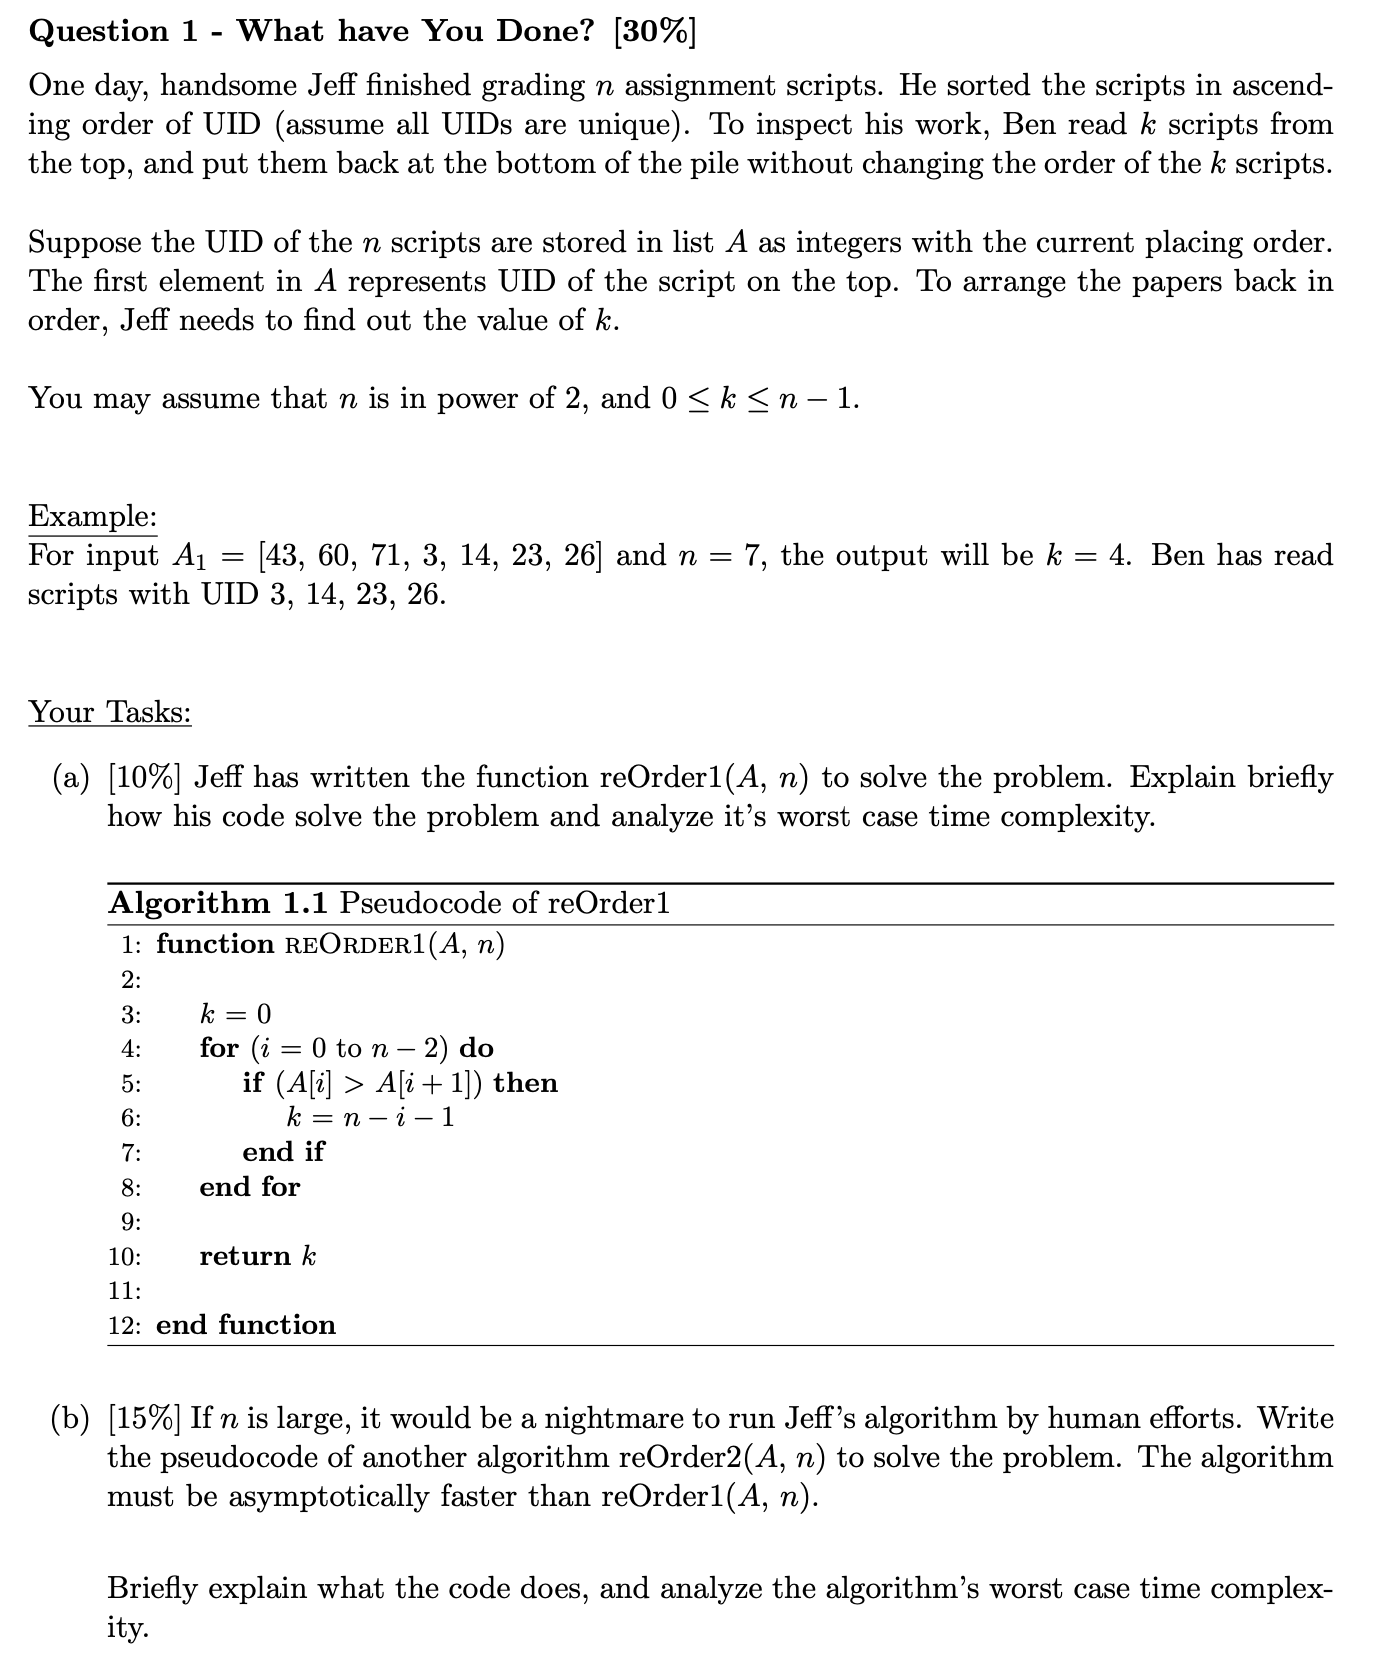
\includegraphics[width=\linewidth]{img/1.png}
\end{center}

\subsection*{(a)}
The function checks from the start of the list A if the number is greater than the next number. If it is, then $k$ is number of elements after the current indice, given by $n-i-1$ where $i$ is the current indice.

It's worst time case complexity is $O(n)$ for when $k$ is 0.

\subsection*{(b)}

\begin{lstlisting}[language=Python]
function REORDER2(A, n)
    if (n <= 1 or A[0] < A[n-1])
        return 0
    left = 0
    right = n - 1
    while (left + 1 < right)
        middle = (left + right) / 2
        if (A[middle] < A[n-1])
            right = middle
        else
            left = middle
    return n - right
\end{lstlisting}

The worst time case complexity is $O(\log n)$, as the search space is halved each time.

The code returns 0 if the list is sorted in ascending order, as there is no read scripts, otherwise, it works by checking if the middle element is less than the last element. If it is, then the pivot point is in the left half of the list (inclusive), otherwise, it's in the right half. This is because the pivot point is the smallest element in the list. We repeat this process until the search space is reduced to 2 elements, at which point we return the index of the smaller element.

\section*{Question 2}

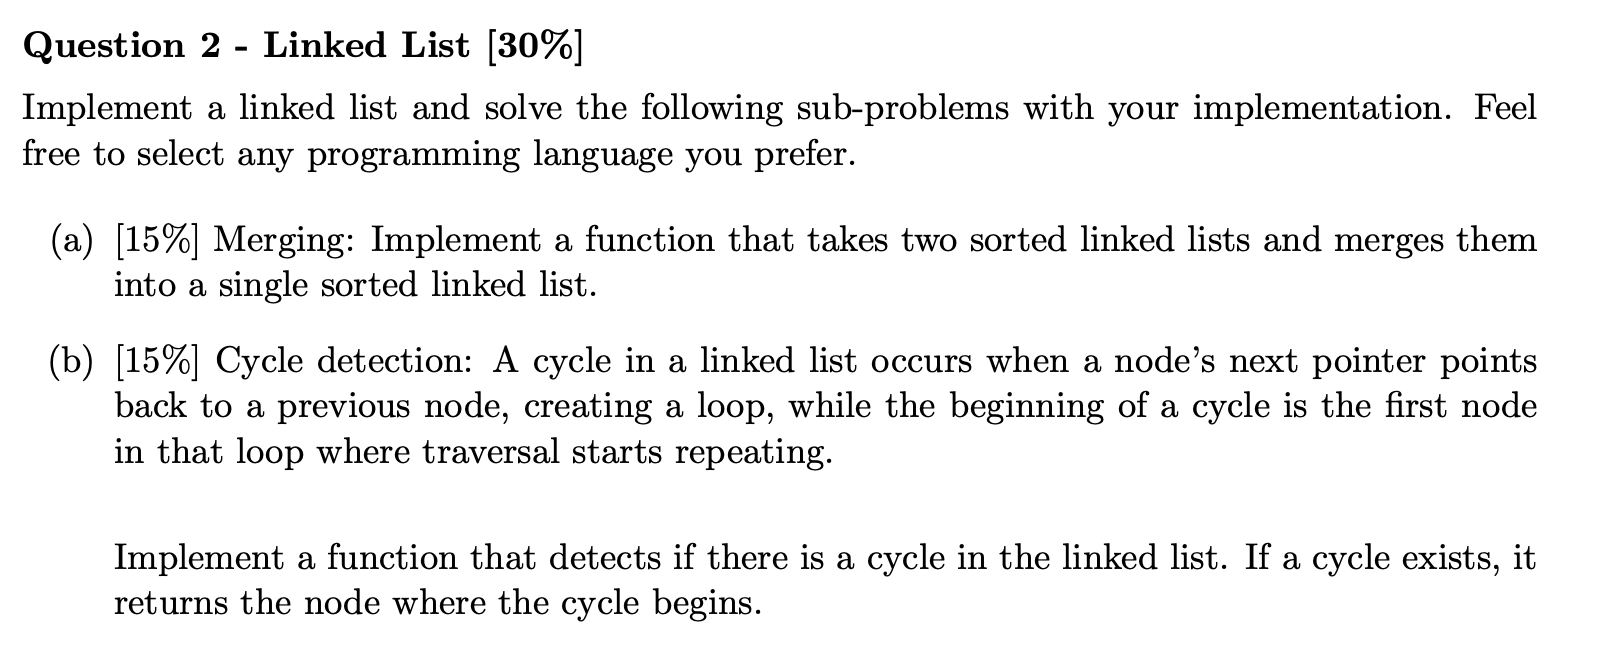
\includegraphics[width=\linewidth]{img/2.png}

\lstinputlisting[language=Java, basicstyle=\footnotesize\ttfamily]{2.js}

\section*{Question 3}

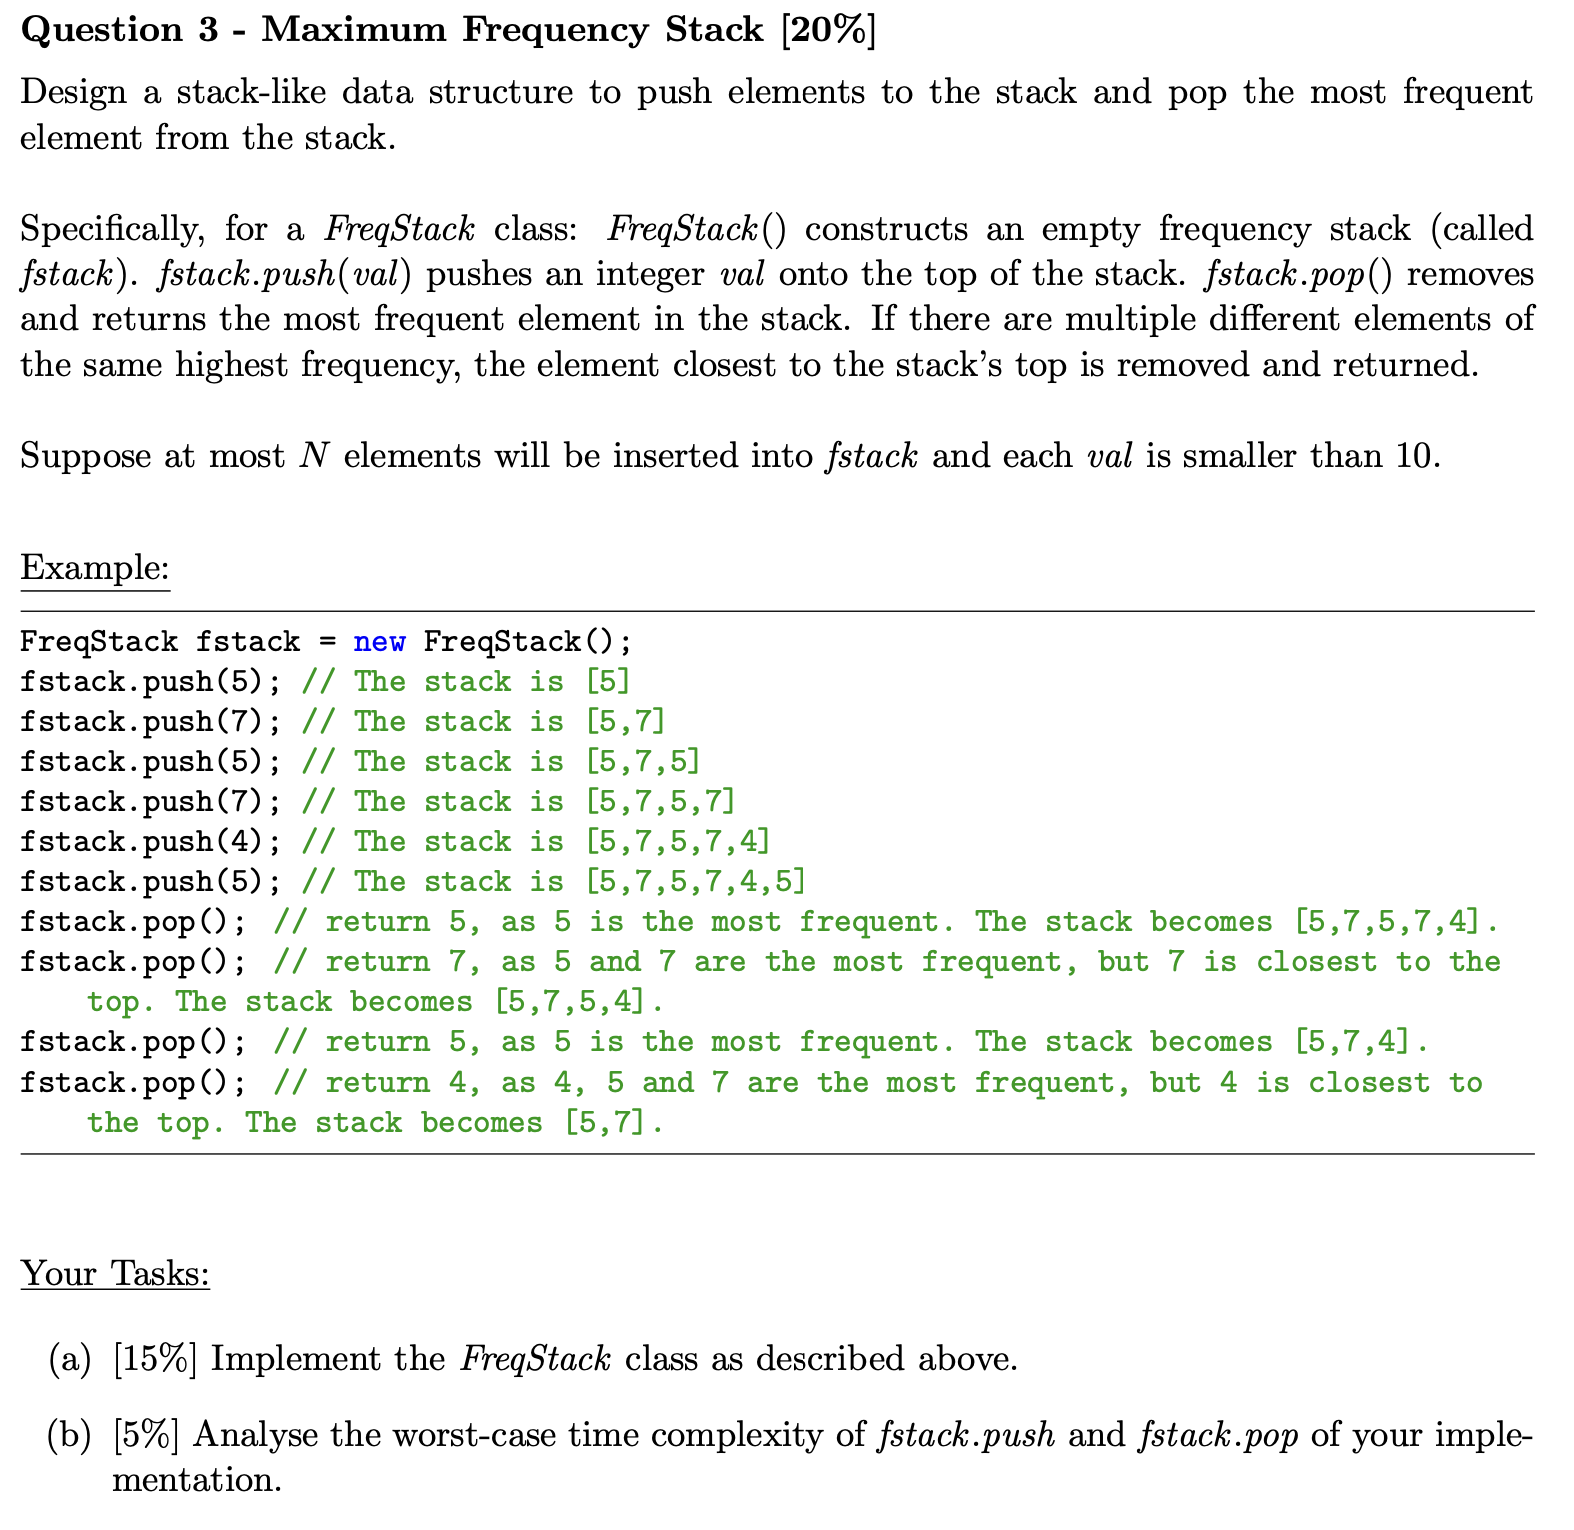
\includegraphics[width=\linewidth]{img/3.png}

\subsection*{(a)}

\lstinputlisting[language=Java, basicstyle=\footnotesize\ttfamily]{3.js}

\subsection*{(b)}

Push: O(1) as we are just adding to the end of the array.

Pop: O(n) as we search through the entire array to find the most frequent element.

\section*{Question 4}

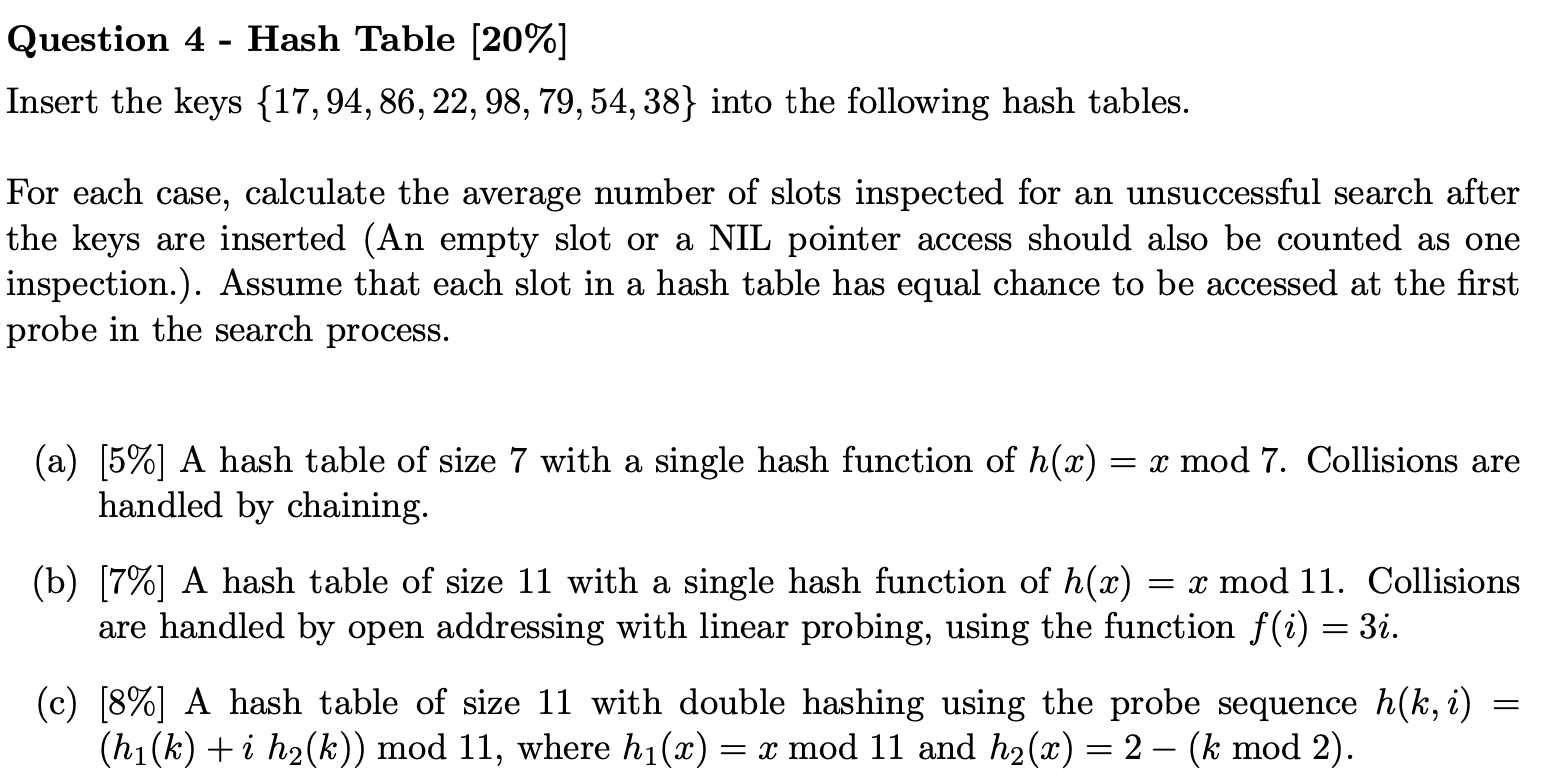
\includegraphics[width=\linewidth]{img/4.png}

\subsection*{(a)}

$m = 7,\quad h(k) = k \mod 7$ with chaining.

\begin{center}
    \begin{tabular}{|c|c|c|c|c|c|c|c|c|}
        \hline
        \textbf{Key}  & 17   & 94   & 86   & 22   & 98   & 79   & 54   & 38   \\
        \hline
        \textbf{Hash} & 3    & 3    & 2    & 1    & 0    & 2    & 5    & 3    \\
        \hline
        \textbf{Slot} & 3[0] & 3[1] & 2[0] & 1[0] & 0[0] & 2[1] & 5[0] & 3[2] \\
        \hline
    \end{tabular}
    \begin{tabular}{|r|l|}
        \hline
        \textbf{Slot} & \textbf{Linked List}            \\
        \hline
        0             & 98 $\to$ null                   \\
        1             & 22 $\to$ null                   \\
        2             & 86 $\to$ 79 $\to$ null          \\
        3             & 17 $\to$ 94 $\to$ 38 $\to$ null \\
        4             & null                            \\
        5             & 54 $\to$ null                   \\
        6             & null                            \\
        \hline
    \end{tabular}
\end{center}

Average number of slots inspected for unsuccessful search: $\frac{8}{7}$

\subsection*{(b)}

$m = 11,\quad h(k) = k \mod 11$ with linear probing $f(i) = 3i$.

\begin{center}
    \begin{tabular}{|c|c|c|c|c|c|c|c|c|c|c|c|c|}
        \hline
        \textbf{Key}  & 17 & 94            & 86            & 22 & 98 & 79 & 54                         & 38            \\
        \hline
        \textbf{Hash} & 6  & 6             & 9             & 0  & 10 & 2  & 10                         & 5             \\
        \hline
        \textbf{Slot} & 6  & \xcancel{6} 9 & \xcancel{9} 1 & 0  & 10 & 2  & \xcancel{10} \xcancel{2} 5 & \xcancel{5} 8 \\
        \hline
    \end{tabular}
    \begin{tabular}{|r|l|}
        \hline
        \textbf{Slot} & \textbf{Value} \\
        \hline
        0             & 22             \\
        1             & 86             \\
        2             & 79             \\
        3             & null           \\
        4             & null           \\
        5             & 54             \\
        6             & 17             \\
        7             & null           \\
        8             & 38             \\
        9             & 94             \\
        10            & 98             \\
        \hline
    \end{tabular}
\end{center}

Average number of slots inspected for unsuccessful search: $\frac1{1-\frac{8}{11}}=\frac{11}3$

\subsection*{(c)}

$m = 11,\quad h(k) = k \mod 11$ with double hashing $f(i) = i \cdot h'(k),\quad h'(k) = 2 - (k \mod 2)$.

\begin{center}
    \begin{tabular}{|c|c|c|c|c|c|c|c|c|c|c|c|c|}
        \hline
        \textbf{Key}  & 17 & 94            & 86 & 22 & 98 & 79 & 54             & 38 \\
        \hline
        \textbf{Hash} & 6  & 6             & 9  & 0  & 10 & 2  & 10             & 5  \\
        \hline
        \textbf{Slot} & 6  & \xcancel{6} 8 & 9  & 0  & 10 & 2  & \xcancel{10} 1 & 5  \\
        \hline
    \end{tabular}
    \begin{tabular}{|r|l|}
        \hline
        \textbf{Slot} & \textbf{Value} \\
        \hline
        0             & 22             \\
        1             & 54             \\
        2             & 79             \\
        3             & null           \\
        4             & null           \\
        5             & 38             \\
        6             & 17             \\
        7             & null           \\
        8             & 94             \\
        9             & 86             \\
        10            & 98             \\
        \hline
    \end{tabular}
\end{center}

Average number of slots inspected for unsuccessful search: $\frac{1}{1-\frac{8}{11}}=\frac{11}3$

\end{document}
